% Corpus distribution charts. Bar heights are the REAL tallies of the 160 catalogue benchmarks
% (year, lane, eval mode, VLA-vs-WM contrast), re-counted from docs/assets/catalog_p3.js.
\begin{figure*}[tp]
\centering
\definecolor{pal1}{HTML}{C0392B}\definecolor{pal2}{HTML}{E67E22}\definecolor{pal3}{HTML}{B7950B}%
\definecolor{pal4}{HTML}{1E8449}\definecolor{pal5}{HTML}{7D3C98}\definecolor{pal6}{HTML}{C2185B}%
\definecolor{pal7}{HTML}{566573}\definecolor{pal8}{HTML}{6E2C00}\definecolor{pal9}{HTML}{7B241C}%
\definecolor{pal10}{HTML}{4A235A}%
\resizebox{\textwidth}{!}{%
\begin{tabular}{@{}c@{\hspace{7mm}}c@{}}
% ---- (a) benchmarks per year ----
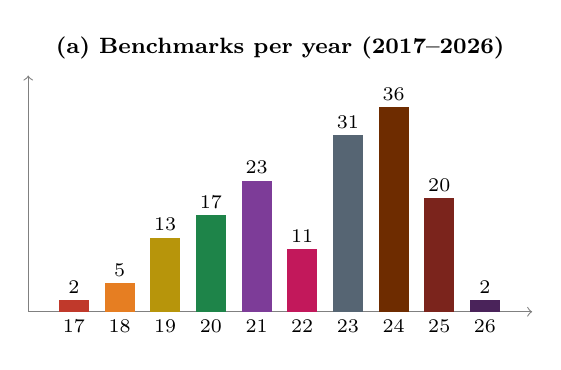
\begin{tikzpicture}[baseline]
  \draw[->,gray] (0,0)--(0,3.0); \draw[->,gray] (0,0)--(6.4,0);
  \foreach [count=\i] \l/\v in {17/2,18/5,19/13,20/17,21/23,22/11,23/31,24/36,25/20,26/2}{
    \fill[pal\i] ({\i*0.58-0.19},0) rectangle ({\i*0.58+0.19},{\v*0.0722});
    \node[font=\scriptsize] at ({\i*0.58},-0.18) {\l};
    \node[font=\scriptsize,above=-1pt] at ({\i*0.58},{\v*0.0722}) {\v};
  }
  \node[font=\footnotesize\bfseries] at (3.2,3.35) {(a) Benchmarks per year (2017--2026)};
\end{tikzpicture}
&
% ---- (b) evaluation lane ----
\begin{tikzpicture}[baseline]
  \draw[->,gray] (0,0)--(0,3.0); \draw[->,gray] (0,0)--(5.0,0);
  \foreach [count=\i] \l/\v/\c in {policy/37/cat-vla, embodied/85/cat-code,
                                    {wm-eval}/34/cat-skill, bridge/4/cat-bench}{
    \fill[\c!75!black] ({\i*1.1-0.3},0) rectangle ({\i*1.1+0.3},{\v*0.0306});
    \node[font=\scriptsize] at ({\i*1.1},-0.18) {\l};
    \node[font=\scriptsize,above=-1pt] at ({\i*1.1},{\v*0.0306}) {\v};
  }
  \node[font=\footnotesize\bfseries] at (2.5,3.35) {(b) Evaluation lane};
\end{tikzpicture}
\\[7mm]
% ---- (c) evaluation mode (horizontal) ----
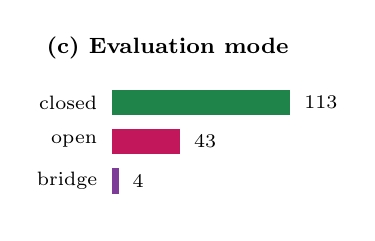
\begin{tikzpicture}[baseline]
  \foreach [count=\i] \l/\v/\c in {closed/113/pal4, open/43/pal6, bridge/4/pal5}{
    \fill[\c] (1.5,{1.75-\i*0.5}) rectangle ({1.5+\v*0.020},{1.75-\i*0.5+0.32});
    \node[left=2pt,font=\scriptsize] at (1.5,{1.75-\i*0.5+0.16}) {\l};
    \node[right=1.5pt,font=\scriptsize] at ({1.5+\v*0.020},{1.75-\i*0.5+0.16}) {\v};
  }
  \node[font=\footnotesize\bfseries] at (2.2,2.1) {(c) Evaluation mode};
\end{tikzpicture}
&
% ---- (d) VLA-vs-WM contrast (horizontal; the thesis panel) ----
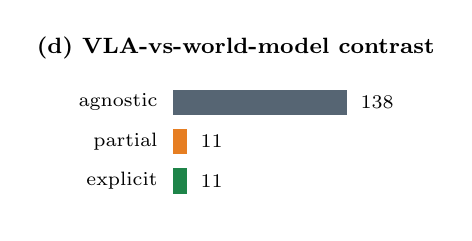
\begin{tikzpicture}[baseline]
  \foreach [count=\i] \l/\v/\c in {agnostic/138/pal7, partial/11/pal2, explicit/11/pal4}{
    \fill[\c] (1.6,{1.75-\i*0.5}) rectangle ({1.6+\v*0.016},{1.75-\i*0.5+0.32});
    \node[left=2pt,font=\scriptsize] at (1.6,{1.75-\i*0.5+0.16}) {\l};
    \node[right=1.5pt,font=\scriptsize] at ({1.6+\v*0.016},{1.75-\i*0.5+0.16}) {\v};
  }
  \node[font=\footnotesize\bfseries] at (2.4,2.1) {(d) VLA-vs-world-model contrast};
\end{tikzpicture}
\end{tabular}}
\caption{\textbf{Profile of the 160 catalogue benchmarks} (Table~\ref{tab:landscape}), re-counted
directly from the catalogue. (a)~publication year, showing the 2023--2024 surge; (b)~evaluation lane
(embodied navigation dominates, then policy suites); (c)~evaluation mode (closed-loop task success
dominates, open-loop prediction is second, only four bridges reach action); (d)~whether the benchmark
builds a native Vision-Language-Action vs world-model contrast, the survey's organising question:
\textbf{138 of 160 are model-agnostic}, and only \textbf{11 (7\%)} build the contrast explicitly.
Counts are the exact column tallies of Table~\ref{tab:landscape}.}
\Description{Four bar charts of the 160 benchmarks. (a) Benchmarks per year rise from 2 in 2017 to 31
in 2023 and 36 in 2024, then 20 in 2025. (b) Evaluation lane: policy 37, embodied 85, world-model
evaluation 34, bridge 4. (c) Evaluation mode: closed 113, open 43, bridge 4. (d) VLA-vs-world-model
contrast: model-agnostic 138, partial 11, explicit 11, with a note that only 11 (7 percent) build a
contrast.}
\label{fig:corpus_dist}
\end{figure*}
